\section{Durchführung des Versuches}
\label{sec:Durchführung}
\subsection{Versuchsaufbau}
Der verwendete Vesuchsaufbau ist in Abbildung \ref{fig:Aufbau} skizziert.
Dieser teilt sich ein einen optischen und einen eletronischen Aufbau auf.
\begin{figure}[H]
    \centering
    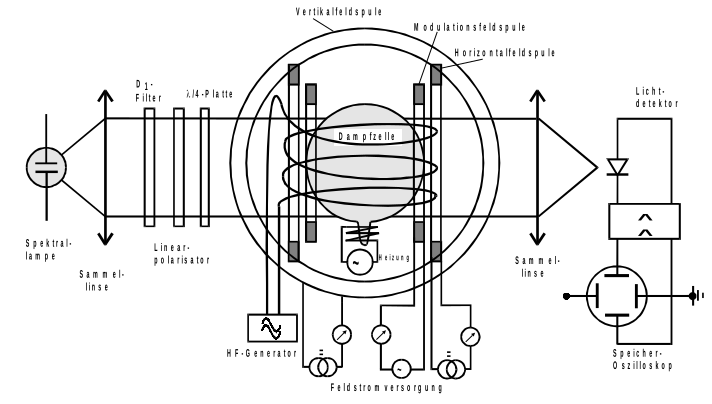
\includegraphics[scale= 0.4]{pictures/aufbau.png}
    \caption{Skizze des Versuchsaufbaus \cite{V21}.}
    \label{fig:Aufbau}
\end{figure}
\noindent
Als Lichtquelle für den optischen Aufbau dient eine Spektrallampe.
Nachdem das Licht duch eine Sammellinse parallelisiert wurde, wird 
mittels Interferenzfilter die $\text{D}_\text{1}$-Linie des 
Rb-Spektrums isoliert. Durch einen Polarisationsfilter und eine 
$\lambda/4$-Platte wird sicher gestellt, dass die Dampfzelle nur mit 
rechts zirkular polarisiertes Licht bestrahlt wird. Um den Dampfdruck 
des Rb-Gases innerhalb der Dampfzelle regulieren zu können, ist die 
Dampfzelle mit einer Heizvorrichtung ausgestattet. 

\noindent
Um die Dampfzelle
herum befindet sich eine Anordnung aus verschiedenen Helmholtz-Spulen.
Zwei vertikal angeordnete Spulen (Horizontalfeld- und Sweep-Spule) und 
eine horizontal angeordnete Vertikalfeldspule zum Ausgleichen der 
Vertikalkomponente des Erdmagnetfeldes. Desweiteren erzeugt die 
RF-Spule ein hochfrequentes Wechselmagnetfeld, welches über einen 
Impulsgenerator in der Frequenz variiert werden kann. 

\noindent
Nachdem das Licht durch eine weitere Sammellinse fokusiert wurde, folgt 
der elektrische Aufbau. Durch einen Photodetektor wird das Lichtsignal
in elektrisches Signal übersetzt. Dieses gelangt dann über einen 
Linearverstäker in ein Oszilloskop und ein Galvanometer. An dem 
Oszilloskop kann die Lichtintensität als elektrisches Signal abgelesen
werden.

\subsection{Durchführung}
Es wird mit der Justage es Strahengangs begonnen, sodass das 
Galvanometer eine maximale Stromstärke misst. Somit ist die 
Lichtintensität auf dem Photodetektor maximal. Danach werden 
alle weiteren optischen Bauelemente im Strahengang montiert und der 
Aufbau vor Restlicht abgeschirmt.

\noindent
Sowohl die Vertikal- als auch die Horizontalfeldspule werden 
ausgeschalet. Der Startwert der Sweep-Spule wird auf null und die 
Range auf den Maximalwert gestellt. Auf dem Oszilloskop wird ein 
breiter Peak abgebildet, dessen Breite es zu minimieren gilt. Dazu 
wird die Orientierung des Aufbaus im Raum und die Stärke der 
Vertikalfeldspule angepasst. Dies dient der Kompensation des 
Erdmagnetfeldes. 

\noindent
Es folgt die Messung der Resonanzfrequenz der beiden Rubidiumisotope.
Die RF-Spule wird mit einer Frequenz von $\SI{100}{\kilo\hertz}$
angeschaltet und mit einem $\SI{4}{\volt}$-Sinus Signal betrieben. 
Die erscheinenden Resonanzfrequenzen sind auf dem Oszilloskop abzulesen. 
Um die Resonanzfrequenz zu vermessen werden die Frequenzen der RF-Spule
in $\SI{100}{\kilo\hertz}$ Schritten bis $\SI{1}{\mega\hertz}$ verändert.
Da das Magentfeld der Sweep-Spule nicht ausreicht, um die Resonanzen
bei jeder Frequenz auf dem Oszilloskop darzustellen, kann mit Hilfe 
der Horizontalfeldspule ein höheres Feld erzeugt werden.